\documentclass[11pt]{article}
\usepackage{etoolbox}
\usepackage[letterpaper,margin=1in]{geometry}
\usepackage[parfill]{parskip}
\usepackage{amsmath,amssymb,graphicx}
\usepackage{fancyhdr}
\usepackage{enumerate}
\usepackage{xcolor}
\usepackage{tikz}

\newcommand{\docdate}{January 16, 2019}
\newcommand{\duedate}{??:00 AM, January ??, 2019 }

\newcommand{\sol}{\bigskip\textbf{Solution.}\qquad\qquad}

\setlength{\headheight}{14pt}
\renewcommand{\baselinestretch}{1.3}
\pagestyle{fancyplain}
\fancyfoot{}
\fancyhead[L]{Homework \HomeworkNo{}}
\fancyhead[C]{OMCIT 592}
\fancyhead[R]{\thepage}
\renewcommand{\headrulewidth}{0pt}
\setlength{\headheight}{14pt}
\setlength{\headsep}{12pt}
\setlength{\footskip}{0pt}

\fancypagestyle{firstpage}{
  \fancyhead{}
  \fancyfoot{}
}


\newcommand{\problembreak}{\bigskip\hrule\bigskip}
\newcommand{\points}[1]{\textbf{[#1 pts]}}

%%%%%%%%%%%%%%%%%%%%%%%%%%%%%%%%%%%%%%
%%%  DO NOT MODIFY ABOVE THIS LINE  %%
%%%%%%%%%%%%%%%%%%%%%%%%%%%%%%%%%%%%%%


\newcommand{\HomeworkNo}{11}


\begin{document}

\thispagestyle{firstpage}

\begin{center}
{\Large OMCIT 592 \hfill Homework \HomeworkNo}\\[20pt]
\fbox{YOUR NAME}
\hfill
\fbox{YOUR EMAIL OR COURSERA ID}
\hfill
\fbox{\today}
\end{center}

\vspace*{2cm}

\problembreak

\vspace*{2cm}


\begin{enumerate}
[\bf 1.]
  \setlength\itemsep{10pt}


%%%%%%%%%%%%%%%%%%%%
%%%  PROBLEM 1  %%%
%%%%%%%%%%%%%%%%%%%%
  
\item \points{10} 
In the \emph{adjacency matrix} of a graph $G=(V,E)$ with $V=\{v_1,v_2,\ldots,v_n\}$, the entry in the $i$\textsuperscript{th} row and the $j$\textsuperscript{th} column is 1 if $\{v_i,v_j\}\in E$ and 0 otherwise. For example, the graph
		\begin{center}
			\begin{tikzpicture}
			\tikzstyle{every node}+=[draw,circle,inner sep=0pt,minimum size=20]
			\node (a) at (0,0) {$1$};
			\node (b) at (0,2) {$2$};
			\node (c) at (2,0) {$3$};
			\node (d) at (2,2) {$4$};
			\draw (a) -- (b) -- (d) -- (c) -- (b);
			\end{tikzpicture}
		\end{center}
		has adjacency matrix
		\[\begin{bmatrix}
		0&1&0&0\\
		1&0&1&1\\
		0&1&0&1\\
		0&1&1&0
		\end{bmatrix}\]
		What is the adjacency matrix of the following graph?
	
		\begin{center}
		\begin{tikzpicture}
		\tikzstyle{every node}+=[draw,circle,inner sep=0pt,minimum size=20]
		\node (a) at (0,0) {$1$};
		\node (b) at (1.5,0) {$2$};
		\node (c) at (2.5,1.25) {$3$};
		\node (d) at (1.5,2.5) {$4$};
		\node (e) at (0,2.5) {$5$};
		\node (f) at (-1,1.25) {$6$};
		\draw (a) -- (b) -- (f);
		\draw (e) -- (b) -- (c) -- (d) -- (e) -- (a);
		\tikzstyle{every node}=[]
		\node (r) at (3.5,0) {};
		\end{tikzpicture}
		
		\end{center}
		
\sol

YOUR SOLUTION HERE

\bigskip

\bigskip



%%%%%%%%%%%%%%%%%%%%
%%%  PROBLEM 2  %%%
%%%%%%%%%%%%%%%%%%%%

\item \points{10} 
Consider a graph with the vertex set
\[\{\text{Thorin, Fili, Kili, Balin, Dwalin, Oin, Gloin, Dori, Nori, Ori, Bifur, Bofur, Bombur}\}\,.\]
Two vertices form an edge in this graph if their names share a 3-letter subsequence. The subsequence does not need to be consecutive, but it does need to be in order. For example, Ba\underline{lin} is adjacent to G\underline{l}o\underline{in}. List the connected components of this graph.

\sol

YOUR SOLUTION HERE

\bigskip

\bigskip



%%%%%%%%%%%%%%%%%%%%
%%%  PROBLEM 3  %%%
%%%%%%%%%%%%%%%%%%%%

\item \points{10} 
Consider the graph whose edges are the seams of a standard soccer ball and whose vertices are the places where these seams meet.

Each vertex in this graph lies at the corner of one of the 12 black pentagons and has degree 3. How many edges are in this graph?

\sol

YOUR SOLUTION HERE

\bigskip

\bigskip


%%%%%%%%%%%%%%%%%%%%
%%%  PROBLEM 4  %%%
%%%%%%%%%%%%%%%%%%%%

\item \points{10} 
A \emph{$d$-regular} graph is a graph in which every vertex has the same degree $d$, where $d$ is some natural number. Prove that there is no 9-regular graph with 42 edges.

\sol

YOUR SOLUTION HERE

\bigskip

\bigskip


%%%%%%%%%%%%%%%%%%%%
%%%  PROBLEM 5  %%%
%%%%%%%%%%%%%%%%%%%%

\item \points{10} 
Prove that every graph with at least two vertices contains two vertices with the same degree.

\sol

YOUR SOLUTION HERE

\bigskip

\bigskip

%%%%%%%%%%%%%%%%%%%%
%%%  PROBLEM 6  %%%
%%%%%%%%%%%%%%%%%%%%

\item \points{10} 
Recall the \textit{divides} relation from earlier in the semester. Given two integers \textit{a} and \textit{b}, we said that \textit{a} divides \textit{b}, written $a~ | ~b$, if there is some integer $k$ such that $a \times k = b$. Prove that this relation is reflexive and transitive but not symmetric.

\sol

YOUR SOLUTION HERE

\bigskip

\bigskip

%%%%%%%%%%%%%%%%%%%%
%%%  PROBLEM 7  %%%
%%%%%%%%%%%%%%%%%%%%

\item \points{6} \textbf{OPTIONAL EXTRA CREDIT PROBLEM}
Li and Rose are married. They invite three other married couples to a party at their house. Various people shake hands during the party, but no one shakes hands with their own spouse (or with themselves, of course). At the end of the party, Li asks everybody else how many people they shook hands with and receives seven different responses. How many people did Rose shake hands with?

\sol

YOUR SOLUTION HERE

\bigskip

\bigskip


\end{enumerate}
\end{document}